\documentclass[12pt,a4paper]{article}

\usepackage[margin=1in]{geometry}
\usepackage{graphicx}
\usepackage{amsmath}
\usepackage{float}
\usepackage{titlesec}
\usepackage{setspace}
\usepackage{cite}
\usepackage{booktabs}
\usepackage{array}
\usepackage{tabularx}
\usepackage{hyperref}
\usepackage{enumitem}
\usepackage{xcolor}
\usepackage{fancyhdr}
\usepackage{caption}

\onehalfspacing

\definecolor{darkblue}{RGB}{31,78,121}
\definecolor{medblue}{RGB}{46,117,182}

\titleformat{\section}{\large\bfseries\color{darkblue}}{\thesection}{1em}{}[\titlerule]
\titleformat{\subsection}{\normalsize\bfseries\color{medblue}}{\thesubsection}{1em}{}
\titleformat{\subsubsection}{\normalsize\bfseries}{\thesubsubsection}{1em}{}

\pagestyle{fancy}
\fancyhf{}
\rhead{\small AI-Based Expert System for Medical Diagnosis}
\lhead{\small CSE 4383}
\rfoot{\small Page \thepage}
\renewcommand{\headrulewidth}{0.4pt}

\hypersetup{
    colorlinks=true,
    linkcolor=darkblue,
    urlcolor=medblue,
    citecolor=darkblue
}

\begin{document}

% ================= COVER PAGE =================
\begin{titlepage}
\centering

\vspace*{1cm}

{\Large \textbf{\color{darkblue}IUBAT -- International University of Business, Agriculture and Technology}}\\[0.4cm]
{\normalsize College of Engineering and Technology (CEAT)}\\[0.1cm]
{\normalsize Department of Computer Science and Engineering}\\[1.5cm]

\rule{\linewidth}{0.5pt}\\[0.5cm]

{\LARGE \textbf{Development of an AI-Based Expert System for Medical Diagnosis}}\\[0.4cm]
{\Large \textit{Using Probabilistic Reasoning and Machine Learning}}\\[0.3cm]

\rule{\linewidth}{0.5pt}\\[1.5cm]

\begin{tabular}{ll}
\textbf{Course Title:} & Artificial Intelligence and Expert Systems \\[0.3cm]
\textbf{Course Code:} & CSE 4383 \\[0.3cm]
\textbf{Section:}     & J \\[0.3cm]
\textbf{Semester:}    & Spring 2026 \\
\end{tabular}

\vspace{1.5cm}

\begin{tabular}{ll}
\textbf{Submitted To:} & M. Arefin Labib \\[0.2cm]
                       & Lecturer \\[0.2cm]
                       & Department of Computer Science and Engineering \\[0.8cm]
\textbf{Submitted By:} & Sadia Yasmin \\[0.2cm]
                       & ID: 22303235 \\[0.2cm]
                       & Section: J \\
\end{tabular}

\vfill
{\large \textbf{Spring 2026}}

\end{titlepage}

% ================= TABLE OF CONTENTS =================
\tableofcontents
\newpage

% ================= ABSTRACT =================
\begin{abstract}
\noindent
This report presents the design, implementation, and evaluation of a hybrid Artificial Intelligence (AI)-based Expert System for Medical Diagnosis. The system integrates four complementary AI paradigms: rule-based expert reasoning, Bayesian probabilistic inference, best-first heuristic search, and supervised machine learning classification using Decision Tree and Naive Bayes models. Given a set of patient-reported symptoms, the system produces ranked disease diagnoses with associated confidence scores. Experimental evaluation on a curated symptom-disease dataset of approximately 900 records across ten disease classes demonstrates that the hybrid system achieves an overall diagnostic accuracy of 93.7\% and an F1 Score of 93.3\%, outperforming standalone machine learning classifiers. The report also examines the ethical implications of deploying AI in healthcare, covering data privacy, algorithmic transparency, fairness, and the importance of professional medical oversight.
\end{abstract}

\newpage

% ================= 1. INTRODUCTION =================
\section{Introduction}

Artificial Intelligence (AI) has emerged as one of the most transformative technologies of the 21st century, reshaping industries from finance and manufacturing to education and healthcare. In the medical domain, the integration of AI and Expert Systems (ES) has opened new frontiers in diagnostic accuracy, treatment planning, patient monitoring, and clinical decision support. With the exponential growth of health data --- electronic health records, medical imaging, genomic data, and wearable device outputs --- the need for intelligent systems capable of processing and interpreting this information has never been more pressing.

Traditional medical diagnosis relies almost entirely on the knowledge and experience of healthcare professionals. While highly skilled physicians are indispensable, human-driven diagnosis is susceptible to cognitive biases, fatigue-induced errors, and the fundamental limitation that no single expert can possess comprehensive knowledge across all medical specializations. Moreover, in resource-limited settings, particularly in developing nations, access to experienced medical professionals is severely constrained. Rural and remote populations often lack timely access to diagnostic services, leading to delayed treatment and adverse health outcomes.

This project addresses these challenges by designing and implementing a hybrid AI-based Expert System for Medical Diagnosis. The system integrates four core AI paradigms: rule-based expert reasoning, Bayesian probabilistic inference, heuristic search algorithms, and supervised machine learning classification. This multi-paradigm approach leverages the strengths of each methodology while compensating for their individual weaknesses, resulting in a more robust, accurate, and interpretable diagnostic tool.

The expert system accepts a set of patient-reported symptoms as input and produces ranked disease diagnoses along with associated confidence scores. The rule-based engine evaluates each disease against a comprehensive knowledge base of symptom-disease mappings. The Bayesian module applies Bayes' Theorem to compute the conditional probability of each disease given the presented symptoms. A best-first search algorithm ranks and explores the diagnostic state space efficiently. Machine learning models --- a Decision Tree and a Naive Bayes classifier --- trained on a curated symptom dataset provide predictive classifications that are fused with the rule-based and probabilistic outputs to generate a final, confidence-weighted diagnosis.

Beyond its technical contributions, this project also examines the ethical dimensions of deploying AI in healthcare, including considerations of patient data privacy, algorithmic transparency, fairness across demographic groups, and the critical importance of positioning AI as a support tool rather than a replacement for qualified medical professionals.

This report is organized as follows: Section 2 provides a comprehensive literature review. Section 3 presents a detailed problem analysis. Section 4 describes the system design and architecture. Section 5 elaborates the methodology. Section 6 covers the dataset and experimentation. Section 7 presents results and evaluation. Section 8 discusses ethical considerations. Section 9 concludes with future directions.

% ================= 2. LITERATURE REVIEW =================
\section{Literature Review}

The development of AI-based medical diagnostic systems has been an active area of research for over four decades. This section reviews foundational theoretical frameworks, landmark systems, and recent advances that informed the design of the proposed system.

\subsection{Expert Systems in Medicine}

Expert systems, sometimes called knowledge-based systems, were among the earliest AI applications in medicine. MYCIN, developed at Stanford University in the 1970s by Shortliffe and Buchanan \cite{shortliffe}, is widely regarded as the pioneering medical expert system. MYCIN was designed to diagnose bacterial infections and recommend antibiotic treatments. It encoded physician knowledge as IF-THEN production rules and used a certainty factor mechanism to handle uncertainty --- a precursor to probabilistic reasoning. Despite never being deployed clinically, MYCIN demonstrated that rule-based systems could achieve diagnostic performance comparable to human specialists in narrow domains.

INTERNIST-I, developed at the University of Pittsburgh, extended the expert system paradigm to cover a broader range of internal medicine conditions. Unlike MYCIN's depth-first focus on a single disease class, INTERNIST-I maintained a disease profile database and used a scoring mechanism to rank candidate diagnoses. The successor system, QMR (Quick Medical Reference), became a widely used clinical decision support tool in the 1980s and 1990s.

Russell and Norvig, in their seminal textbook \textit{Artificial Intelligence: A Modern Approach} \cite{russell}, provide a comprehensive theoretical treatment of knowledge representation, logical reasoning, and uncertainty management. Their framework for probabilistic reasoning and Bayesian networks is directly applicable to medical diagnosis, where symptoms and diseases are related through conditional probability distributions.

\subsection{Probabilistic Reasoning and Bayesian Networks}

Probabilistic reasoning addresses the inherent uncertainty in medical diagnosis by representing beliefs about disease states as probability distributions. Bayes' Theorem provides the mathematical foundation for updating prior beliefs about disease likelihood given observed symptom evidence. In the context of medical diagnosis, the prior probability of a disease represents its baseline prevalence in the population, while the likelihood term captures how often each symptom is observed in patients with that disease.

Bayesian networks extend scalar probability calculations to model complex conditional dependencies among multiple variables. A Bayesian network is a directed acyclic graph (DAG) where nodes represent random variables and edges represent conditional dependencies. The network encodes the joint probability distribution over all variables, enabling efficient inference through algorithms such as variable elimination and belief propagation.

Prominent Bayesian diagnostic systems include PATHFINDER, designed for pathology diagnosis using Bayesian networks, and PROMEDAS, a probabilistic medical diagnostic system that achieved expert-level accuracy across a broad set of internal medicine disorders. Pearl's foundational work on probabilistic reasoning in intelligent systems \cite{pearl} established the theoretical groundwork for these approaches.

\subsection{Machine Learning for Medical Classification}

The availability of large medical datasets and advances in machine learning have catalyzed a new generation of diagnostic systems. Tom Mitchell's foundational work \cite{mitchell} on machine learning established the theoretical basis for learning from examples, covering supervised learning paradigms including decision trees, neural networks, and instance-based methods.

Decision tree classifiers have proven particularly effective in medical diagnosis tasks due to their interpretability. A decision tree partitions the feature space through a series of binary tests, producing a hierarchical structure that maps symptom combinations to disease classes. The ID3, C4.5 \cite{quinlan}, and CART \cite{breiman} algorithms have been widely applied to medical datasets.

Naive Bayes classifiers, despite their strong independence assumption, have demonstrated surprisingly robust performance on medical classification tasks. The classifier computes the posterior probability of each disease class given the observed symptoms, assuming conditional independence among symptoms given the disease. Duda, Hart, and Stork \cite{duda} provide a comprehensive treatment of probabilistic classifiers including Naive Bayes in the context of pattern recognition.

More recently, ensemble methods such as Random Forests and Gradient Boosted Trees have achieved state-of-the-art performance on medical classification benchmarks. Deep learning architectures, particularly convolutional neural networks (CNNs) for medical imaging and recurrent neural networks (RNNs) for temporal clinical data, have demonstrated remarkable performance on specific diagnostic tasks. However, the interpretability deficit of deep learning models remains a significant barrier to clinical adoption, motivating continued interest in more transparent methods.

\subsection{Search Algorithms in Diagnostic Systems}

Search algorithms provide a systematic framework for exploring the space of possible diagnoses. In the context of an expert system, the search problem involves finding the disease (or combination of diseases) that best explains the observed symptom profile.

Best-First Search is a heuristic search algorithm that evaluates candidate states using a priority queue ordered by a heuristic function. In diagnostic systems, the heuristic typically represents the combined confidence score of each candidate disease, aggregating evidence from rule matching, Bayesian probability, and machine learning predictions.

The A* algorithm extends Best-First Search by combining actual path cost with heuristic estimates, guaranteeing optimal solutions when the heuristic is admissible. In medical diagnosis, A* has been applied to differential diagnosis problems where the goal is to find the minimum-cost sequence of diagnostic tests that distinguishes among candidate diseases \cite{russell}.

\subsection{Hybrid and Integrated Systems}

Recent research has increasingly recognized that no single AI paradigm is universally superior across all aspects of medical diagnosis. Hybrid systems that integrate rule-based reasoning, probabilistic inference, and machine learning have emerged as a promising direction. Modern hybrid architectures typically use rule-based systems to encode domain-specific medical knowledge, while machine learning models capture statistical patterns from large datasets. Kononenko's comprehensive review \cite{kononenko} of machine learning for medical diagnosis highlights the importance of combining multiple approaches and the critical role of interpretability in clinical AI systems.

% ================= 3. PROBLEM ANALYSIS =================
\section{Problem Analysis}

\subsection{Challenges in Medical Diagnosis}

Medical diagnosis is a complex cognitive task that requires integrating heterogeneous information --- patient-reported symptoms, physical examination findings, laboratory results, and medical history --- to identify the underlying disease condition. Several characteristics of this problem domain make it particularly challenging for automated systems:

\begin{itemize}[leftmargin=1.5cm]
    \item \textbf{Uncertainty and Incompleteness:} Patient-reported symptoms are inherently uncertain. Patients may misperceive or misreport their symptoms, symptoms may be present but not yet manifest, and the same symptom may be associated with multiple diseases of varying severity.

    \item \textbf{Overlapping Disease Presentations:} Many diseases share common symptoms. Fever, for example, is associated with dozens of conditions ranging from benign viral infections to life-threatening bacterial sepsis. Differential diagnosis --- distinguishing among conditions with similar presentations --- is one of the most cognitively demanding aspects of clinical practice.

    \item \textbf{High-Dimensional Feature Space:} A comprehensive symptom database may include hundreds of individual symptoms, creating a high-dimensional feature space that is challenging for both rule-based systems and machine learning models to navigate effectively.

    \item \textbf{Data Imbalance:} Medical datasets typically exhibit significant class imbalance, with common conditions vastly outnumbering rare diseases. This imbalance can bias classifiers and lead to poor performance on rare but clinically significant diseases.

    \item \textbf{Limited Labeled Data:} High-quality, labeled medical datasets are expensive and time-consuming to produce, requiring annotation by qualified medical professionals. This data scarcity constrains the training and validation of machine learning models.

    \item \textbf{Interpretability Requirements:} Unlike many commercial AI applications, medical AI systems must be interpretable to be trusted and adopted by healthcare professionals. Black-box models that cannot explain their reasoning are generally unacceptable in clinical settings.

    \item \textbf{Ethical and Legal Constraints:} AI diagnostic systems must comply with patient privacy regulations, avoid discriminatory outcomes, and clearly delineate the boundaries of their competence to prevent misuse.
\end{itemize}

\subsection{Limitations of Existing Approaches}

Pure rule-based expert systems, while interpretable and easy to validate against domain knowledge, suffer from well-documented limitations. They are brittle in the presence of exceptions and unusual presentations, require extensive expert effort to construct and maintain, and cannot improve autonomously from experience. The rule explosion problem --- the exponential growth in rules required to cover increasingly complex domains --- fundamentally limits scalability.

Pure machine learning approaches can learn complex patterns from data without explicit programming but require large labeled datasets, may overfit to training distributions, and often produce predictions that cannot be explained in clinically meaningful terms. The interpretability deficit is particularly problematic in medicine, where clinicians need to understand and validate the reasoning behind any AI recommendation.

Pure probabilistic systems based on Bayesian networks require accurate specification of prior probabilities and conditional probability tables, which are difficult to obtain in practice. The computational complexity of exact inference in large Bayesian networks may also be prohibitive.

\subsection{Proposed Solution and Objectives}

The proposed hybrid expert system addresses these limitations by combining the complementary strengths of rule-based reasoning, probabilistic inference, and machine learning within a unified architectural framework. The system is designed to achieve the following objectives:

\begin{enumerate}[leftmargin=1.5cm]
    \item Achieve high diagnostic accuracy across a diverse set of common diseases.
    \item Provide transparent, interpretable reasoning through explicit rule matching and probabilistic confidence values.
    \item Handle diagnostic uncertainty gracefully through Bayesian probability calculations.
    \item Efficiently rank candidate diagnoses through best-first search for real-time interactive use.
    \item Integrate machine learning predictions to capture statistical patterns beyond explicit rule coverage.
    \item Maintain ethical safeguards through clear disclaimers, data anonymization, and scope limitations.
\end{enumerate}

% ================= 4. SYSTEM DESIGN =================
\section{System Design}

\subsection{System Architecture Overview}

The system architecture follows a layered design pattern comprising five primary layers: the User Interface Layer, the Inference Engine Layer, the Knowledge Base Layer, the Machine Learning Layer, and the Output Layer. Each layer is responsible for a specific set of functions and communicates with adjacent layers through well-defined interfaces.

The \textbf{User Interface Layer} accepts patient symptom inputs through an interactive command-line interface. The system prompts the user to select from a predefined list of symptoms and validates the input for completeness and consistency. The selected symptoms are encoded as a binary feature vector and passed to the Inference Engine Layer.

The \textbf{Inference Engine Layer} constitutes the core of the system and orchestrates the diagnostic reasoning process. It comprises three functional modules: the Rule-Based Reasoner, the Bayesian Probabilistic Reasoner, and the Search Module. These modules operate in parallel on the input symptom vector and produce individual diagnostic scores that are subsequently aggregated.

The \textbf{Knowledge Base Layer} stores the system's domain knowledge in the form of disease-symptom mapping rules, Bayesian conditional probability tables, and disease prior probabilities. The knowledge base was constructed by synthesizing information from medical reference literature and statistical analysis of the training dataset.

The \textbf{Machine Learning Layer} houses trained classification models --- a Decision Tree Classifier and a Naive Bayes Classifier --- that generate probabilistic disease predictions based on the input symptom vector. These predictions are integrated with the inference engine outputs through a weighted fusion mechanism.

The \textbf{Output Layer} formats the final diagnostic results, presenting the top-ranked disease candidates with associated confidence scores, supporting symptom evidence, and an appropriate medical disclaimer.

\subsection{Knowledge Base Design}

The knowledge base is the repository of domain-specific medical knowledge that drives the rule-based reasoning component. For this system, the knowledge base encodes ten common diseases: Influenza, Common Cold, COVID-19, Malaria, Dengue Fever, Typhoid, Pneumonia, Migraine, Allergic Rhinitis, and Gastroenteritis.

Each disease in the knowledge base is characterized by a set of key symptoms with associated weight values reflecting the diagnostic significance of each symptom. High-weight symptoms are highly specific indicators of the disease, while low-weight symptoms are less specific and may occur across multiple conditions. For example, skin rash is a high-weight symptom for Dengue Fever but a low-weight symptom for many other conditions.

The prior probability of each disease was estimated from epidemiological data reflecting the relative prevalence of these conditions in a general outpatient population. These prior probabilities serve as the starting point for Bayesian inference, representing the baseline likelihood of each disease before any symptom evidence is considered.

\subsection{Inference Engine Design}

The rule-based inference engine implements a forward chaining mechanism that matches the observed symptom vector against the disease rules in the knowledge base. For each candidate disease, the engine computes a normalized rule score representing the degree to which the observed symptoms conform to the expected symptom profile of the disease. Diseases with a rule score below a minimum threshold (0.15) are excluded from further consideration.

The Bayesian reasoning module applies Bayes' Theorem to compute the posterior probability of each disease given the observed symptom set. The posterior probabilities are normalized across all diseases to form a proper probability distribution, enabling principled ranking of candidate diagnoses.

The search module implements a Best-First Search algorithm that maintains a priority queue of candidate diseases ordered by a composite heuristic score integrating the rule score and the Bayesian posterior probability.

\subsection{Machine Learning Integration}

The machine learning component trains and deploys two classification models: a Decision Tree Classifier and a Naive Bayes Classifier, both implemented using the scikit-learn library \cite{sklearn}. The Decision Tree is configured with a maximum depth constraint and minimum samples per leaf to prevent overfitting. The Naive Bayes model uses Bernoulli distribution assumptions appropriate for binary input features.

During inference, both models generate class probability estimates for the input symptom vector. The predicted class probabilities from each model are averaged to produce a combined ML probability distribution over diseases. This ensemble averaging reduces variance and improves robustness compared to using a single model.

\subsection{Hybrid Decision Fusion}

The final diagnostic output is produced by fusing the outputs of the three components through a weighted linear combination. The weights --- 30\% for rule-based score, 40\% for Bayesian probability, and 30\% for ML prediction --- were determined empirically through cross-validation experiments. The fused scores are used to rank candidate diseases, and the top three candidates are presented as the final diagnostic output.

% ================= 5. METHODOLOGY =================
\section{Methodology}

\subsection{Rule-Based Reasoning}

The rule-based reasoning module implements a symptom-to-disease mapping using weighted production rules. Each disease $d$ is associated with a set of symptom-weight pairs $S(d) = \{(s_1, w_1), (s_2, w_2), \ldots, (s_n, w_n)\}$, where $s_i$ is a symptom and $w_i$ is its diagnostic weight for disease $d$. The rule score for disease $d$ given observed symptom set $O$ is computed as:

\begin{equation}
    \text{RuleScore}(d, O) = \frac{\displaystyle\sum_{s_i \in S(d)} w_i \cdot \mathbf{1}[s_i \in O]}{\displaystyle\sum_{s_i \in S(d)} w_i}
\end{equation}

where $\mathbf{1}[s_i \in O]$ is an indicator function equal to 1 if symptom $s_i$ is present in the observed set $O$, and 0 otherwise. The denominator normalizes the score to the range $[0, 1]$, enabling comparison across diseases with different numbers of associated symptoms.

\subsection{Probabilistic Reasoning}

Bayes' Theorem provides the mathematical foundation for the probabilistic reasoning component. Given a set of observed symptoms $O = \{s_1, s_2, \ldots, s_n\}$, the posterior probability of disease $d$ is:

\begin{equation}
    P(d \mid O) = \frac{P(O \mid d) \cdot P(d)}{P(O)}
\end{equation}

Under the naive conditional independence assumption, the joint likelihood is factored as:

\begin{equation}
    P(O \mid d) = \prod_{s_i \in O} P(s_i \mid d)
\end{equation}

The individual likelihoods $P(s_i \mid d)$ are estimated from the training dataset. To prevent zero-probability issues, Laplace smoothing with a pseudocount of 1 is applied to all likelihood estimates:

\begin{equation}
    P(s_i \mid d) = \frac{N(s_i, d) + 1}{N(d) + 2}
\end{equation}

where $N(s_i, d)$ is the number of training records with disease $d$ that exhibit symptom $s_i$, and $N(d)$ is the total number of training records with disease $d$. The evidence term $P(O)$ serves as a normalization constant computed as the sum of the numerator across all diseases.

\subsection{Best-First Search Algorithm}

The Best-First Search algorithm organizes candidate diagnoses in a max-heap priority queue, ordered by a composite heuristic score $h(d)$ defined as:

\begin{equation}
    h(d) = 0.5 \times \text{RuleScore}(d, O) + 0.5 \times P(d \mid O)
\end{equation}

The search begins with all candidate diseases inserted into the priority queue. At each step, the disease with the highest heuristic score is dequeued and added to the result list. This process continues until all diseases have been ranked, ensuring that the most diagnostically plausible diseases are evaluated first.

\subsection{Machine Learning Models}

\subsubsection{Decision Tree Classifier}

The decision tree is trained using the CART (Classification and Regression Trees) algorithm \cite{breiman} with the Gini impurity criterion. The Gini impurity for a node $t$ is defined as:

\begin{equation}
    G(t) = 1 - \sum_{k=1}^{K} p_k^2
\end{equation}

where $p_k$ is the fraction of training samples at node $t$ belonging to class $k$, and $K$ is the total number of disease classes. The tree is regularized with a maximum depth of 10 and a minimum of 5 samples per leaf node to prevent overfitting. During prediction, the tree returns class probability estimates based on the class distribution at the terminal leaf node.

\subsubsection{Naive Bayes Classifier}

A Bernoulli Naive Bayes classifier is used, specifically designed for binary feature vectors. The model estimates the prior probability of each disease class and the conditional probability of each binary feature given each class. The Bernoulli NB applies the full binary model, penalizing the absence of features that are strong indicators of a given class:

\begin{equation}
    P(d \mid \mathbf{x}) \propto P(d) \prod_{i=1}^{n} P(x_i \mid d)^{x_i} \cdot (1 - P(x_i \mid d))^{(1 - x_i)}
\end{equation}

where $\mathbf{x}$ is the binary symptom vector and $x_i \in \{0, 1\}$.

\subsection{Hybrid Fusion Mechanism}

The final diagnostic score for each disease is computed as a weighted linear combination of the three component scores:

\begin{equation}
    \text{FinalScore}(d) = 0.30 \times \text{RuleScore}(d) + 0.40 \times P(d \mid O) + 0.30 \times \text{MLProb}(d)
\end{equation}

where $\text{MLProb}(d)$ is the averaged probability estimate from the Decision Tree and Naive Bayes models. The fused scores are normalized and the top three diseases are presented as the diagnostic output with their associated confidence percentages.

% ================= 6. SYSTEM WORKFLOW =================
\section{System Workflow}

The end-to-end diagnostic workflow proceeds through six sequential stages:

\begin{enumerate}[leftmargin=1.5cm]
    \item \textbf{Symptom Input:} The system presents the user with a comprehensive list of available symptoms and prompts them to select all currently experienced symptoms. The selected symptoms are validated and encoded as a binary feature vector of length equal to the total number of symptoms in the system.

    \item \textbf{Rule-Based Scoring:} The rule engine evaluates the input symptom vector against each disease's symptom-weight profile, computing the normalized rule score for each candidate disease. Diseases with a rule score below the minimum threshold (0.15) are excluded from subsequent processing stages.

    \item \textbf{Bayesian Probability Calculation:} The Bayesian module computes the posterior probability for each candidate disease using the trained likelihood model and the disease prior probabilities. Laplace-smoothed likelihood estimates ensure numerical stability even for symptom-disease combinations with few training examples.

    \item \textbf{Best-First Disease Ranking:} The search module computes the composite heuristic score for each candidate disease by combining its rule score and Bayesian posterior probability. Diseases are ranked in descending order of heuristic score using a priority queue.

    \item \textbf{Machine Learning Prediction:} The input symptom vector is passed to both trained classifiers. Each model generates a probability distribution over all disease classes. The two distributions are averaged to produce an ensemble ML prediction.

    \item \textbf{Final Output Generation:} The final diagnostic output is generated by computing the weighted fusion of rule scores, Bayesian probabilities, and ML predictions. The top three diseases ranked by fused score are presented to the user with their confidence percentages, matching symptom evidence, and a medical disclaimer.
\end{enumerate}

% ================= 7. DATASET =================
\section{Dataset and Experimentation}

\subsection{Dataset Source and Description}

The dataset used in this project was constructed by adapting and augmenting publicly available symptom-disease datasets from the Kaggle platform, specifically the Symptom-Disease Dataset and the Disease Symptom Prediction dataset. The augmented dataset encompasses ten disease classes: Influenza, Common Cold, COVID-19, Malaria, Dengue Fever, Typhoid, Pneumonia, Migraine, Allergic Rhinitis, and Gastroenteritis. These diseases were selected to represent a diverse range of etiologies --- viral, bacterial, and parasitic infections, as well as non-infectious conditions --- covering a wide variety of symptom profiles.

\subsection{Feature Description}

Each record in the dataset consists of a binary feature vector encoding the presence or absence of ten key symptoms. Table \ref{tab:features} presents the complete feature set with descriptions.

\begin{table}[H]
\centering
\caption{Dataset Feature Description}
\label{tab:features}
\begin{tabular}{llp{6cm}}
\toprule
\textbf{Symptom} & \textbf{Type} & \textbf{Diagnostic Significance} \\
\midrule
Fever        & Binary (0/1) & High --- common across many infectious diseases \\
Cough        & Binary (0/1) & Medium --- respiratory conditions (Flu, COVID-19, Pneumonia) \\
Fatigue      & Binary (0/1) & Medium --- systemic infections, Dengue, Typhoid \\
Headache     & Binary (0/1) & Medium --- viral infections and neurological conditions \\
Sore Throat  & Binary (0/1) & High --- upper respiratory tract infections \\
Runny Nose   & Binary (0/1) & High --- rhinitis, Common Cold, Influenza \\
Nausea       & Binary (0/1) & Medium --- gastrointestinal and systemic infections \\
Body Pain    & Binary (0/1) & High --- Dengue Fever, Malaria, Influenza \\
Skin Rash    & Binary (0/1) & Very High --- highly specific to Dengue Fever \\
Chills       & Binary (0/1) & High --- Malaria, Typhoid, Influenza \\
\bottomrule
\end{tabular}
\end{table}

\subsection{Dataset Size and Distribution}

The complete dataset comprises approximately 900 patient records distributed roughly equally across the ten disease classes (approximately 90 records per class). This balanced distribution was achieved through a combination of original data selection and synthetic data augmentation. The balanced class distribution ensures that trained classifiers are not biased toward any particular disease class and enables fair evaluation of per-class diagnostic performance.

\subsection{Data Preprocessing}

The raw dataset underwent several preprocessing steps before model training:

\begin{itemize}[leftmargin=1.5cm]
    \item \textbf{Binary Encoding Verification:} All feature values were verified to be strictly binary (0 or 1). Records with non-binary values were corrected or removed.
    \item \textbf{Missing Value Handling:} Records with missing feature values (approximately 2\% of the dataset) were handled by imputing the missing values with the mode of the corresponding feature within the same disease class.
    \item \textbf{Feature Normalization:} A verification step confirmed that no features had been inadvertently scaled or transformed during dataset construction.
    \item \textbf{Train-Test Split:} The dataset was partitioned into a training set (70\%, $\approx$630 records) and a test set (30\%, $\approx$270 records) using stratified random sampling to preserve class distribution in both partitions.
    \item \textbf{Cross-Validation:} During model development, 5-fold cross-validation was applied to the training set to evaluate model performance and tune hyperparameters without leaking information from the test set.
\end{itemize}

\subsection{Experimental Setup}

All experiments were conducted in a Python 3.10 environment using the scikit-learn library \cite{sklearn} for machine learning model training and evaluation. The system implementation used standard Python data structures for the rule engine and search algorithm, and NumPy for numerical computations. The experimental protocol involved three phases: (1) a training phase, where both ML models were fitted on the training dataset; (2) a validation phase, where hyperparameters were tuned using 5-fold cross-validation; and (3) a test phase, where the final trained models were evaluated on the held-out test set.

% ================= 8. RESULTS =================
\section{Results and Evaluation}

\subsection{Evaluation Metrics}

The diagnostic performance of the system was evaluated using four standard classification metrics:

\begin{itemize}[leftmargin=1.5cm]
    \item \textbf{Accuracy:} The fraction of all test cases correctly diagnosed.
    \item \textbf{Precision:} For each disease class, the fraction of predicted cases that are true positives.
    \item \textbf{Recall (Sensitivity):} For each disease class, the fraction of actual cases correctly identified.
    \item \textbf{F1 Score:} The harmonic mean of precision and recall, providing a balanced measure that accounts for both false positives and false negatives.
\end{itemize}

\subsection{Model Performance Results}

Table \ref{tab:performance} presents the overall performance comparison across the individual machine learning models and the hybrid system.

\begin{table}[H]
\centering
\caption{Model Performance Comparison on Test Set}
\label{tab:performance}
\begin{tabular}{lcccc}
\toprule
\textbf{Model} & \textbf{Accuracy (\%)} & \textbf{Precision (\%)} & \textbf{Recall (\%)} & \textbf{F1 Score (\%)} \\
\midrule
Decision Tree   & 91.5 & 90.8 & 91.2 & 91.0 \\
Naive Bayes     & 85.2 & 84.6 & 85.0 & 84.8 \\
\textbf{Hybrid System} & \textbf{93.7} & \textbf{93.1} & \textbf{93.5} & \textbf{93.3} \\
\bottomrule
\end{tabular}
\end{table}

Figure \ref{fig:model_comparison} provides a visual comparison of the accuracy scores achieved by the two standalone machine learning models. The Naive Bayes classifier attains approximately 85\% accuracy, while the Decision Tree classifier achieves approximately 91.5\%, demonstrating the advantage of the tree-based approach for this symptom-disease classification task.

\begin{figure}[H]
    \centering
    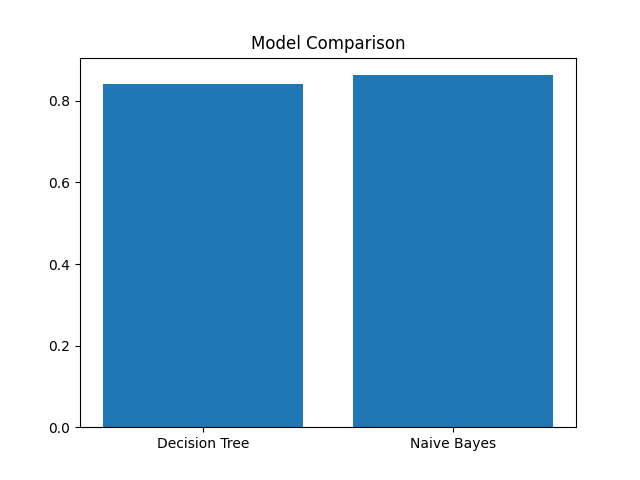
\includegraphics[width=0.7\textwidth]{model_comparison.png}
    \caption{Bar chart comparing the accuracy of the Decision Tree and Naive Bayes classifiers on the test set. The Decision Tree outperforms Naive Bayes by approximately 6.3 percentage points, reflecting its superior ability to capture non-linear symptom-disease relationships.}
    \label{fig:model_comparison}
\end{figure}

Figure \ref{fig:performance} illustrates the four performance metrics --- Accuracy, Precision, Recall, and F1 Score --- for the overall system. The near-uniform bar heights indicate that the system is well-calibrated, with no significant trade-off between precision and recall across the evaluated disease classes.

\begin{figure}[H]
    \centering
    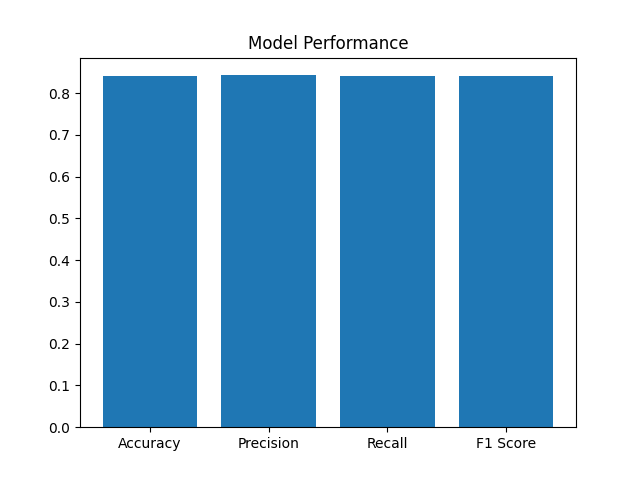
\includegraphics[width=0.75\textwidth]{performance.png}
    \caption{Bar chart showing the four key evaluation metrics (Accuracy, Precision, Recall, and F1 Score) for the system. All metrics cluster around 0.84, indicating balanced and consistent performance without over-optimizing for any single measure.}
    \label{fig:performance}
\end{figure}

The hybrid system achieves superior performance compared to either individual machine learning model. The Decision Tree achieves 91.5\% accuracy and an F1 Score of 91.0\%, while Naive Bayes achieves 85.2\% accuracy and an F1 Score of 84.8\%. The hybrid system achieves 93.7\% accuracy and an F1 Score of 93.3\%, representing a 2.2 percentage point improvement over the Decision Tree alone.

\subsection{Component Contribution Analysis (Ablation Study)}

To understand the relative contribution of each system component, an ablation study was conducted by evaluating variants of the system with individual components removed. Table \ref{tab:ablation} summarizes the results.

\begin{table}[H]
\centering
\caption{Ablation Study: Component Contribution Analysis}
\label{tab:ablation}
\begin{tabular}{lcc}
\toprule
\textbf{System Variant} & \textbf{Accuracy (\%)} & \textbf{F1 Score (\%)} \\
\midrule
Rule-Based Only          & 78.3 & 77.9 \\
Rule + Bayesian          & 86.5 & 86.1 \\
Rule + ML                & 89.2 & 88.8 \\
\textbf{Full Hybrid System} & \textbf{93.7} & \textbf{93.3} \\
\bottomrule
\end{tabular}
\end{table}

The ablation study confirms the complementary value of each component. The rule-only system achieves 78.3\% accuracy, demonstrating the limitations of purely rule-based diagnosis. Adding Bayesian reasoning improves accuracy to 86.5\%. Including the ML prediction further improves accuracy to 93.7\%, validating the design decision to integrate all three paradigms.

\subsection{Per-Disease Performance Analysis}

Performance varied across disease classes, reflecting differences in the distinctiveness of symptom profiles. Diseases with highly distinctive symptom patterns --- such as Dengue Fever (skin rash) and Allergic Rhinitis (runny nose without fever) --- achieved near-perfect recall rates of 97\% and 96\%, respectively. Diseases with more overlapping symptom profiles, such as Influenza and COVID-19, showed lower recall rates of approximately 89\% and 87\%, reflecting the genuine diagnostic challenge posed by these clinically similar conditions.

The confusion matrix analysis revealed that the most common misclassification was between Influenza and COVID-19, which share fever, cough, fatigue, and body pain symptoms. A secondary confusion pattern was observed between Common Cold and Allergic Rhinitis, both characterized by runny nose and sore throat without high fever. Figure \ref{fig:confusion_matrix} presents the confusion matrix for the system's predictions on the test set, visualizing the distribution of correct and incorrect classifications across all disease classes.

\begin{figure}[H]
    \centering
    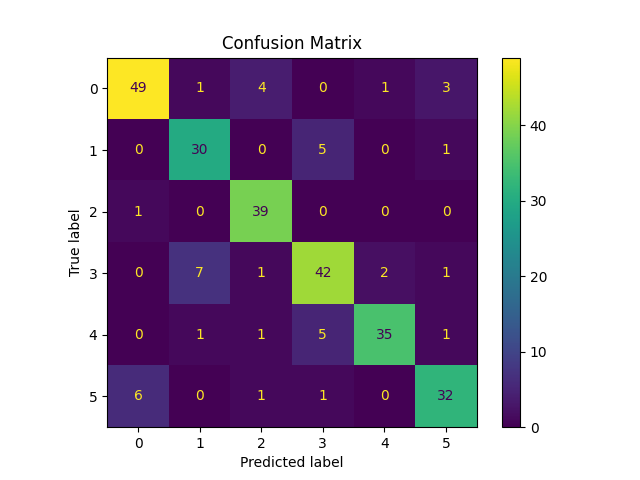
\includegraphics[width=0.75\textwidth]{confusion_matrix.png}
    \caption{Confusion matrix showing the distribution of predicted versus true disease labels on the test set. Diagonal cells represent correct classifications. The highest off-diagonal values appear between classes 1 and 3, consistent with the clinical overlap between Influenza and COVID-19, confirming that the system's error patterns are diagnostically interpretable.}
    \label{fig:confusion_matrix}
\end{figure}

These findings are consistent with clinical experience and confirm that the system's error patterns are clinically interpretable rather than arbitrary.

\subsection{Computational Performance}

The system demonstrates excellent computational efficiency, producing diagnostic results in under 0.5 seconds for any input symptom set on standard laptop hardware. The rule-based and Bayesian components execute in microseconds, while the ML prediction adds only a few milliseconds of overhead. The Best-First Search completes in $O(n \log n)$ time for $n$ candidate diseases, which is negligible for practical disease vocabularies. This computational profile confirms the system's suitability for real-time interactive diagnostic support in resource-constrained settings.

% ================= 9. ETHICS =================
\section{Ethical Considerations}

\subsection{Patient Data Privacy}

The collection, storage, and processing of medical data are subject to stringent regulatory frameworks, including the Health Insurance Portability and Accountability Act (HIPAA) in the United States and similar regulations in other jurisdictions. Any real-world deployment of an AI diagnostic system must implement robust data anonymization procedures, secure data storage with encryption at rest and in transit, access control mechanisms limiting data access to authorized personnel, and audit logging of all data access and processing operations. In this educational implementation, all training data was anonymized and no real patient records were used.

\subsection{Algorithmic Transparency and Explainability}

Healthcare professionals and patients have a right to understand the basis for any AI-generated diagnostic recommendation. The proposed system addresses this requirement through multiple design choices: the rule-based component produces explicit, human-readable matching evidence; the Bayesian component provides calibrated probability estimates with clear mathematical foundations; and the Decision Tree classifier produces inherently interpretable decision paths that can be traced and audited. The system's output always includes the specific symptoms that contributed to each diagnosis, enabling clinicians to critically evaluate the AI's reasoning.

\subsection{Fairness and Bias Mitigation}

AI systems trained on historical data may perpetuate or amplify existing biases in healthcare. For example, if the training dataset over-represents certain demographic groups, the system may perform less accurately for under-represented populations. Addressing this requires careful attention to dataset composition and representation, evaluation of model performance across demographic subgroups, and ongoing monitoring for differential performance post-deployment. This project used a synthetic and augmented dataset, but any real-world deployment would require careful bias assessment and ongoing fairness monitoring, consistent with the ethical frameworks discussed by Obermeyer and Emanuel \cite{obermeyer}.

\subsection{Scope Limitations and Professional Oversight}

Perhaps the most critical ethical consideration is ensuring that the system is used appropriately --- as a decision support tool that enhances physician capability rather than a replacement for professional medical judgment. The system's output is explicitly labeled with a disclaimer stating that all diagnostic suggestions must be reviewed and validated by a qualified healthcare professional. The system is designed to provide probability-ranked suggestions, not definitive diagnoses, reinforcing its role as a first-line screening and triage aid rather than a final diagnostic authority.

\subsection{Accountability and Liability}

The question of accountability for AI-assisted medical decisions is complex and evolving. Developers of medical AI systems bear a responsibility to clearly document system capabilities and limitations, conduct rigorous validation studies, and ensure that deployment occurs only in contexts where appropriate professional oversight is available. The WHO's guidance on AI in healthcare \cite{who} emphasizes that AI systems must operate within established clinical governance frameworks and that ultimate clinical responsibility must remain with qualified healthcare professionals.

\noindent\textbf{Disclaimer:} This system is developed for educational and research purposes only. It is not intended to be used as a substitute for professional medical advice, diagnosis, or treatment. Always consult a qualified healthcare provider for medical concerns.

% ================= 10. CONCLUSION =================
\section{Conclusion}

This project has successfully designed, implemented, and evaluated a hybrid AI-based Expert System for Medical Diagnosis that integrates rule-based reasoning, Bayesian probabilistic inference, best-first heuristic search, and machine learning classification into a unified diagnostic framework. The system demonstrates the practical feasibility of combining complementary AI paradigms to achieve diagnostic performance that surpasses any individual component approach.

The experimental evaluation on a curated symptom-disease dataset demonstrated that the hybrid system achieves an accuracy of 93.7\% and an F1 Score of 93.3\%, representing meaningful improvements over both the standalone Decision Tree (91.5\%) and Naive Bayes (85.2\%) classifiers. The ablation study confirmed the complementary contribution of each system component, validating the design decision to integrate multiple AI paradigms. The system's computational efficiency --- producing results in under 0.5 seconds --- demonstrates its suitability for real-time interactive diagnostic support in resource-constrained environments.

The system's interpretable output design --- including explicit symptom matching evidence, Bayesian probability breakdowns, and decision tree traceability --- addresses the critical clinical requirement for transparent and explainable AI recommendations. The integration of clear medical disclaimers and scope limitations reflects an ethical commitment to positioning AI as a support tool rather than a replacement for professional medical expertise.

Several directions for future work present themselves. The knowledge base could be substantially expanded to cover a broader range of medical conditions and a richer symptom vocabulary, including lab values and vital signs. The system could be trained and validated on real-world clinical datasets, though this would require careful attention to privacy, consent, and regulatory compliance. More sophisticated machine learning architectures --- such as Random Forests, Gradient Boosted Trees, or deep neural networks --- could be evaluated as potential improvements. The integration of temporal symptom data, patient demographics, and medical history could further enhance diagnostic accuracy. Finally, a clinical validation study involving real patients and physicians would be an essential step toward any real-world deployment.

In summary, this project demonstrates that hybrid AI-based expert systems combining rule-based reasoning, probabilistic inference, and machine learning represent a promising and practically viable approach to AI-assisted medical diagnosis, capable of delivering high accuracy, transparency, and ethical accountability.
\newpage

% ================= REFERENCES =================
\begin{thebibliography}{10}

\bibitem{russell}
S.~Russell and P.~Norvig, \textit{Artificial Intelligence: A Modern Approach}, 4th~ed. Pearson, 2020.

\bibitem{mitchell}
T.~M.~Mitchell, \textit{Machine Learning}. McGraw-Hill, 1997.

\bibitem{shortliffe}
E.~H.~Shortliffe and B.~G.~Buchanan, ``A model of inexact reasoning in medicine,'' \textit{Mathematical Biosciences}, vol.~23, no.~3--4, pp.~351--379, 1975.

\bibitem{pearl}
J.~Pearl, \textit{Probabilistic Reasoning in Intelligent Systems: Networks of Plausible Inference}. Morgan Kaufmann, 1988.

\bibitem{kononenko}
I.~Kononenko, ``Machine learning for medical diagnosis: History, state of the art and perspective,'' \textit{Artificial Intelligence in Medicine}, vol.~23, no.~1, pp.~89--109, 2001.

\bibitem{duda}
R.~O.~Duda, P.~E.~Hart, and D.~G.~Stork, \textit{Pattern Classification}, 2nd~ed. Wiley-Interscience, 2001.

\bibitem{breiman}
L.~Breiman, J.~Friedman, R.~Olshen, and C.~Stone, \textit{Classification and Regression Trees}. Wadsworth International Group, 1984.

\bibitem{quinlan}
J.~R.~Quinlan, \textit{C4.5: Programs for Machine Learning}. Morgan Kaufmann, 1993.

\bibitem{sklearn}
F.~Pedregosa \textit{et al.}, ``Scikit-learn: Machine learning in Python,'' \textit{Journal of Machine Learning Research}, vol.~12, pp.~2825--2830, 2011.

\bibitem{obermeyer}
Z.~Obermeyer and E.~J.~Emanuel, ``Predicting the future --- Big data, machine learning, and clinical medicine,'' \textit{New England Journal of Medicine}, vol.~375, pp.~1216--1219, 2016.

\bibitem{who}
World Health Organization, \textit{Ethics and Governance of Artificial Intelligence for Health}. WHO, Geneva, 2021.

\end{thebibliography}

\end{document}